% =============================================================================
% Supporting Information
% Quantum Agrivoltaic Digital Twin: Coordinated Vibronic Light-Harvesting,
% Environmental Calibration, and Agro-Rural Cybersecurity
% Target: Nature Energy
% Date:    June 18, 2026 (First Draft)
% Authors: Teguia Kouam S.C., Goumai Vedekoi T., Tchapet Njafa J.-P.,
%          Nguenang J.-P., Nana Engo S.G.
% =============================================================================

\documentclass[11pt,a4paper]{article}

% ---- Required packages ----
\usepackage[utf8]{inputenc}
\usepackage[T1]{fontenc}
% siunitx MUST be loaded before physics to prevent \qty conflict
% (physics defines \qty as absolute-value/bra-ket; siunitx defines \qty{val}{unit})
\usepackage{siunitx}
\usepackage{amsmath,amssymb,amsfonts,graphicx,booktabs,physics,bm,multirow}
\usepackage[version=4]{mhchem}
\DeclareSIUnit{\yr}{yr}
\DeclareSIUnit{\kB}{kB}
\DeclareSIUnit{\USD}{USD}
\DeclareSIUnit{\tonne}{t}
\DeclareSIUnit{\ha}{ha}
\DeclareSIUnit{\hectare}{ha}
\DeclareSIUnit{\MWh}{MWh}
\DeclareSIUnit{\cubed}{^{3}}
\DeclareSIUnit{\nM}{nM}
\DeclareSIUnit{\molar}{M}
\DeclareSIUnit{\minute}{min}
\DeclareSIUnit{\ppb}{ppb}
\DeclareSIUnit{\day}{d}
\usepackage{xcolor}
\usepackage[margin=2.5cm]{geometry}
\usepackage[colorlinks=true,linkcolor=blue,citecolor=blue,urlcolor=blue]{hyperref}
\usepackage[capitalise,nameinlink]{cleveref}
\usepackage{authblk}
\usepackage{xr}
\usepackage{enumitem}

% ---- Cross-reference to main manuscript ----
% \externaldocument{Manuscript_NatureEnergy_26-06-25}

% ---- siunitx v3/v4 configuration ----
\sisetup{
    locale = US,
    detect-all = true,
    group-minimum-digits = 4,
    separate-uncertainty = true,
    multi-part-units = single,
    range-phrase = {--},
    range-units = single,
    quantity-product = \,,
}

% Restore siunitx \qty{value}{unit} after physics package overwrites it.
% (siunitx v3+ omits \qty when physics is detected; this re-instates it.)
% See siunitx manual §3.1: "Interaction with the physics package".
\AtBeginDocument{\RenewCommandCopy\qty\SI}

\emergencystretch 2em

% ---- SI numbering conventions ----
\renewcommand{\theequation}{S\arabic{equation}}
\renewcommand{\thefigure}{S\arabic{figure}}
\renewcommand{\thetable}{S\arabic{table}}
\renewcommand{\thesection}{S\arabic{section}}

% =============================================================================
% DOCUMENT
% =============================================================================

\newcommand{\eqphift}{\Cref{eq:SI_phi_ft}}

\begin{document}

\title{\textbf{Supporting Information}\\[0.5em]
\large Quantum Agrivoltaic Digital Twin: Coordinated Vibronic Light-Harvesting, Environmental Calibration, and Agro-Rural Cybersecurity}

\author{Steve Cabrel Teguia Kouam}
\affil{Department of Physics, Faculty of Science, University of Douala, Cameroon}
\author{Theodore Goumai Vedekoi}
\affil{Department of Physics, Faculty of Science, University of Yaound\'{e}~I, Cameroon}
\author{Jean-Pierre Tchapet Njafa}
\affil{Department of Physics, Faculty of Science, University of Yaound\'{e}~I, Cameroon}
\author{Penabei Samafou}
\affil{Department of Medical Imaging and Radiation Sciences, Faculty of Medicine and Health Sciences, Université de Sherbrooke, 3001, 12th Avenue Nord, Sherbrooke, QC J1H 5N4, Canada}
\author{Jean-Pierre Nguenang}
\affil{Department of Physics, Faculty of Science, University of Douala, Cameroon}
\author{Serge Guy Nana Engo}
\affil{Department of Physics, Faculty of Science, University of Yaound\'{e}~I, Cameroon}
\author{Corresponding author: \texttt{steve.teguia@facsciences-uy1.cm}}

\date{\today}

\maketitle

\noindent\textbf{Associated Manuscript:}
This Supporting Information accompanies the manuscript ``Coordinated Vibronic Light-Harvesting and Polaritonic Interface for Symbiotic Quantum Agrivoltaics'' submitted to \textit{Nature Energy}.
Equations, figures, and tables are prefixed with ``S'' (e.g., Eq.~S1, Fig.~S1, Table~S1).
References to the main manuscript are indicated by unadorned equation/figure numbers (e.g., Eq.~1, Fig.~1).

\vspace{1em}

\tableofcontents

\newpage

%==============================================================================
% SECTION S1: 8-SITE FMO HAMILTONIAN AND COUPLING PARAMETERS
%==============================================================================

\section{8-Site FMO hamiltonian and full coupling matrix}
\label{SI-sec:hamiltonian}

\subsection{Hamiltonian formulation}

The 8-site Fenna--Matthews--Olson (FMO) Hamiltonian used throughout this work extends the standard 7-site model~\cite{Adolphs2006} by including the eighth bacteriochlorophyll $a$ molecule that bridges the chlorosome baseplate to the reaction center~\cite{Moix2011}.
The full electronic Hamiltonian in the site basis is:

\begin{equation}
\hat{H}_{\mathrm{FMO}} = \sum_{n=1}^{8} \varepsilon_n \dyad{n} + \sum_{n \neq m} J_{nm} \dyad{n}{m} - i\Gamma_{\mathrm{RC}} \sum_{j \in \{3,4\}} \dyad{j}{j},
\label{eq:SI_fmo_hamiltonian}
\end{equation}

where $\varepsilon_n$ are the site energies (referenced to the lowest-energy site), $J_{nm}$ are the inter-site electronic couplings, and $\Gamma_{\mathrm{RC}} = \qty{0.15}{\per\ps}$ is the irreversible reaction center trapping rate applied to Sites~3 and~4.
The anti-Hermitian term $-i\Gamma_{\mathrm{RC}}$ models irreversible charge separation at the reaction center; the Hamiltonian is non-Hermitian only on these diagonal trapping terms.

\subsection{Site energies}

\Cref{tab:SI_site_energies} lists the site energies used in all production simulations.
Energies are given relative to the lowest-energy site (Site~3 at \qty{12210}{\per\cm}) and are expressed in \unit{\per\cm}.

\begin{table}[htbp]
\centering
\caption{\textbf{8-site FMO site energies} (in \unit{\per\cm}, referenced to Site~3).}
\label{tab:SI_site_energies}
\begin{tabular}{l *{8}{S[table-format=5.0]} }
\toprule
\textbf{Parameter} & {\textbf{Site 1}} & {\textbf{Site 2}} & {\textbf{Site 3}} & {\textbf{Site 4}} & {\textbf{Site 5}} & {\textbf{Site 6}} & {\textbf{Site 7}} & {\textbf{Site 8}} \\
\midrule
Absolute $\varepsilon_n$ & 12410 & 12530 & 12210 & 12320 & 12480 & 12630 & 12440 & 12410 \\
Relative $\varepsilon_n$ & 280   & 420   & 0     & 110   & 270   & 500   & 310   & 200   \\
\bottomrule
\end{tabular}
\end{table}

The absolute site energies are taken from the Adolphs--Renger parameterization~\cite{Adolphs2006} for Sites~1--7.
Site~8, which bridges the baseplate to the reaction center, is assigned an energy of \qty{12410}{\per\cm} based on the eighth-bacteriochlorophyll characterization by Moix~\textit{et al.}~\cite{Moix2011}.

\subsection{Electronic coupling matrix}

\Cref{tab:SI_coupling_matrix} presents the full $8\times8$ electronic coupling matrix $J_{nm}$ (in \unit{\per\cm}).
The matrix is symmetric ($J_{nm} = J_{mn}$), and all 28 unique coupling pairs are listed.
Values for Sites~1--7 follow the Adolphs--Renger parameterization~\cite{Adolphs2006}; couplings involving Site~8 are taken from~Ref.~\cite{Moix2011}.\begin{table}[htbp]
\centering
\caption{\textbf{Full 8-site electronic coupling matrix $J_{nm}$} (in \unit{\per\cm}).}
\label{tab:SI_coupling_matrix}
\begin{tabular}{l *{8}{S[table-format=-2.1]} }
\toprule
 & {\textbf{Site 1}} & {\textbf{Site 2}} & {\textbf{Site 3}} & {\textbf{Site 4}} & {\textbf{Site 5}} & {\textbf{Site 6}} & {\textbf{Site 7}} & {\textbf{Site 8}} \\
\midrule
\textbf{Site 1} & 0 & -87.7 & 5.5  & -5.9 & 6.7  & -13.7 & -9.9 & 4.0 \\
\textbf{Site 2} & {}  & 0     & 30.8 & 8.2  & 0.7  & 11.8  & 4.3  & -2.1 \\
\textbf{Site 3} & {}  & {}      & 0    & -53.5 & -2.2 & -9.6  & 6.0  & 12.0 \\
\textbf{Site 4} & {}  & {}      & {}     & 0    & -70.7 & -17.0 & -63.3 & 5.5 \\
\textbf{Site 5} & {}  & {}      & {}     & {}     & 0    & 81.1  & -1.3 & 3.2 \\
\textbf{Site 6} & {}  & {}      & {}     & {}     & {}     & 0     & 39.7 & -8.7 \\
\textbf{Site 7} & {}  & {}      & {}     & {}     & {}     & {}      & 0    & -15.0 \\
\textbf{Site 8} & {}  & {}      & {}     & {}     & {}     & {}      & {}     & 0 \\
\bottomrule
\end{tabular}
\end{table}e}

\subsection{Reaction center trapping}

The irreversible trapping is implemented through a non-Hermitian term on Sites~3 and~4, which together form the primary funnel to the reaction center in the 8-site FMO model~\cite{Renger2003,Moix2011}.
The trapping rate $\Gamma_{\mathrm{RC}} = \qty{0.15}{\per\ps}$ corresponds to a trapping time of $\tau_{\mathrm{RC}} \approx \qty{6.7}{\ps}$, consistent with ultrafast charge separation rates measured in reaction center complexes~\cite{Renger2003}.
The forward transfer yield is defined as:

\begin{equation}
\Phi_{\mathrm{FT}} = 2\Gamma_{\mathrm{RC}} \int_0^{t_{\mathrm{max}}} \left[ P_3(t) + P_4(t) \right] dt,
\label{eq:SI_phi_ft}
\end{equation}

with $t_{\mathrm{max}} = \qty{1}{\ps}$ and $P_j(t) = \rho_{jj}(t)$.
The factor of 2 accounts for the two trapping sites.

\subsection{Hermiticity validation}

The non-Hermiticity is strictly confined to the diagonal entries of Sites~3 and~4.
For all $i \neq j$, $H_{ij} = H_{ji}^*$ is satisfied within machine precision (\num{1e-14}).
The Hamiltonian's Hermiticity condition is verified for all 64 matrix elements at every time step of the simulation.

%==============================================================================
% SECTION S2: CONVERGENCE ANALYSIS
%==============================================================================

\section{Convergence analysis}
\label{SI-sec:convergence}

\subsection{Hierarchy depth convergence}
We adopt $L=8$ as the production standard to ensure robust convergence across all disorder realizations. The numerical framework (PT-HOPS/SBD implementation, hierarchy equations) is directly inherited from the validation framework established in Paper~I~\cite{Kouam2026}, where convergence was validated via MAE analysis on the same excitonic parameters.

\Cref{tab:SI_hierarchy_convergence} summarizes the mean absolute error (MAE) between successive $L$ values and the relative deviation from the $L=9$ reference (computed for a subset of 10 disorder realizations).

\begin{table}[htbp]
\centering
\caption{\textbf{Hierarchy depth convergence.} MAE between successive hierarchy depths for exciton populations, averaged over all 8 sites and 100 disorder realizations.}
\label{tab:SI_hierarchy_convergence}
\begin{tabular}{S[table-format=1.0] S[table-format=1.1e-2] S[table-format=1.1e-2] S[table-format=1.1]}
\toprule
{$L$} & {MAE ($L \to L+1$)} & {Rel.\ dev.\ from $L=9$} & {CPU time (min)} \\
\midrule
6 & 9.8e-10 & 1.2e-8 & 2.1 \\
7 & 9.6e-10 & 1.1e-8 & 4.3 \\
8 & 3.1e-11 & 4.2e-10 & 7.5 \\
\bottomrule
\end{tabular}
\end{table}

The MAE between $L=7$ and $L=8$ is $\num{3.1e-11}$, which is below double-precision round-off for most observables.
We adopt $L=8$ as the production standard to ensure robust convergence across all disorder realizations.

\subsection{Matsubara truncation}

We test Matsubara term counts $K = 1, 2, 3$ to assess the impact of high-temperature corrections.
\Cref{tab:SI_matsubara_convergence} shows the effect on the coherence lifetime $\tau_c$ and the forward transfer yield $\Phi_{\mathrm{FT}}$.

\begin{table}[htbp]
\centering
\caption{\textbf{Matsubara truncation convergence.} Impact of $K$ on key observables at \qty{295}{\kelvin}.}
\label{tab:SI_matsubara_convergence}
\begin{tabular}{S[table-format=1.0] S[table-format=3.2(2)] S[table-format=1.2(1)] S[table-format=1.1e-1]}
\toprule
{$K$} & {$\tau_c$ (fs)} & {$\Phi_{\mathrm{FT}}$} & {MAE from $K=3$} \\
\midrule
1 & 406(30) & 0.86(3) & 3.4e-4 \\
2 & 420(35) & 0.89(3) & 3.3e-5 \\
3 & 422(36) & 0.89(3) & {---} \\
\bottomrule
\end{tabular}
\end{table}

The MAE between $K=2$ and $K=3$ is $\num{3.3e-5}$, confirming that $K=2$ is sufficient for converged dynamics at room temperature.
This is consistent with the expectation that at \qty{295}{\kelvin}, the dynamics are dominated by the explicit vibronic modes rather than high-order Matsubara corrections to the Drude--Lorentz background.

\subsection{Time step convergence}

We verify time step convergence by comparing $\Delta t = \qtylist{0.2;1.0;2.0}{\fs}$.
\Cref{tab:SI_timestep_convergence} summarizes the results.

\begin{table}[htbp]
\centering
\caption{\textbf{Time step convergence.} Maximum population deviation relative to the $\Delta t = \qty{0.2}{\fs}$ reference.}
\label{tab:SI_timestep_convergence}
\begin{tabular}{S[table-format=1.1] S[table-format=1.1e-1]}
\toprule
{$\Delta t$ (fs)} & {Max.\ population deviation} \\
\midrule
0.2 & {--- (reference)} \\
1.0 & 4.3e-3 \\
2.0 & 8.1e-3 \\
\bottomrule
\end{tabular}
\end{table}

We adopt $\Delta t = \qty{0.2}{\fs}$ as the production standard, consistent with Paper~I~\cite{Kouam2026}.

\subsection{Detailed balance}

The steady-state populations are compared with the analytical Boltzmann distribution to verify detailed balance.
The maximum deviation across all 8 sites is \qty{2.3}{\percent}, confirming that thermal equilibrium is correctly reproduced.

\subsection{Physical consistency checks}

All production simulations satisfy the following consistency checks:
\begin{itemize}
\item \textbf{Trace preservation:} $\max_t |\Tr[\rho(t)] - 1| < \num{1e-12}$
\item \textbf{Positivity:} $\min_i \lambda_i(t) > -\num{1e-14}$ for all eigenvalues $\lambda_i$ of $\rho(t)$
\item \textbf{Hermiticity:} $\max_{i,j,t} |\rho_{ij}(t) - \rho_{ji}^*(t)| < \num{1e-14}$
\item \textbf{Population realness:} $\max_{i,t} |\Im[\rho_{ii}(t)]| < \num{1e-14}$
\end{itemize}

%==============================================================================
% SECTION S3: POLARON DRESSING MECHANISM
%==============================================================================

\section{Polaron dressing mechanism and residual reorganization energy}
\label{SI-sec:polaron}

\subsection{Canonical (lang--firsov) transformation}

The polaron dressing mechanism that underlies the coherence protection reported in the main text can be rigorously understood through the canonical Lang--Firsov transformation~\cite{Chin2013,Huelga2013}.
The full system-bath Hamiltonian is:

\begin{equation}
\hat{H} = \hat{H}_S + \sum_n \dyad{n} \sum_k g_{n,k}(\hat{b}_{n,k}^\dagger + \hat{b}_{n,k}) + \hat{H}_{\mathrm{bath}},
\label{eq:SI_full_hamiltonian}
\end{equation}

where $g_{n,k}$ are the system-bath coupling constants for mode $k$ at site $n$, and $\hat{b}_{n,k}$ ($\hat{b}_{n,k}^\dagger$) are the bath annihilation (creation) operators.

The unitary transformation $\hat{U} = \exp\!\left[\sum_n \dyad{n} \sum_k \frac{g_{n,k}}{\omega_k}(\hat{b}_{n,k}^\dagger - \hat{b}_{n,k})\right]$ partially diagonalizes the system-bath coupling.
After applying $\hat{U}$, the transformed Hamiltonian becomes:

\begin{equation}
\hat{H}' = \hat{U}^\dagger \hat{H} \hat{U} = \hat{H}_S' + \hat{H}_{\mathrm{bath}} + \hat{H}_{\mathrm{res}},
\label{eq:SI_lf_hamiltonian}
\end{equation}

where $\hat{H}_S'$ contains renormalized excitonic couplings (the polaron-shifted energies) and $\hat{H}_{\mathrm{res}}$ represents the residual system-bath coupling after the transformation.

\subsection{Residual spectral density}

The key physical insight is that underdamped vibronic modes satisfying the resonance condition $\Delta E_{nm} \approx \hbar\omega_v \pm J_{nm}$ become partially ``dressed'' by the canonical transformation: they are incorporated into $\hat{H}_S'$ and no longer contribute to dephasing in the transformed frame.
The residual spectral density is:

\begin{equation}
J_{\mathrm{res}}(\omega) = J_{\mathrm{bath}}(\omega) - \sum_{k \in \mathcal{S}} \frac{\lambda_k \omega_k^2 \gamma_k}{(\omega - \omega_k)^2 + \gamma_k^2},
\label{eq:SI_residual_spectral}
\end{equation}

where $\mathcal{S}$ denotes the set of underdamped modes that are vibronically dressed.

\subsection{Quantitative effect}

For the 12-mode Kleinekath\"{o}fer/Coker parameterization at \qty{295}{\kelvin}, the residual reorganization energy under the two excitation scenarios is:

\begin{align}
\lambda_{\mathrm{res}}^{\mathrm{broad}} &= \lambda_{\mathrm{DL}} + \sum_{k=1}^{12} S_k \omega_k \approx \qty{53}{\per\cm}, \label{eq:SI_lambda_broad} \\
\lambda_{\mathrm{res}}^{\mathrm{filt}} &= \lambda_{\mathrm{DL}} + \sum_{k \notin \mathcal{S}} S_k \omega_k \approx \qty{40}{\per\cm}. \label{eq:SI_lambda_filt}
\end{align}

The \qty{20}{\percent} reduction in $\lambda_{\mathrm{res}}$ translates to a \qty{50}{\percent} coherence lifetime extension (since $\tau_c \propto 1/\lambda_{\mathrm{res}}$ in the high-temperature limit).
The dual-band filter at \qty{750}{\nm} and \qty{820}{\nm} selectively excites those vibronic resonances that are most strongly coupled to the energy-transfer pathway (primarily the \qty{180}{\per\cm} Franck--Condon mode at Sites~3/4 and the \qty{740}{\per\cm} ring deformation mode), maximizing the dressing effect.

\subsection{Connection to PT-HOPS/SBD}

In the PT-HOPS/SBD simulation framework, this protection is captured natively: the bath correlation function is decomposed into Drude--Lorentz and underdamped components, and the hierarchy equations propagate the system-bath entanglement without assuming weak coupling.
The resulting trajectories exhibit the suppressed decoherence predicted by the vibronic-basis analysis when the pulse spectrum matches the underdamped resonances.

%==============================================================================
% SECTION S4: DYNAMIC PHOTO-PROTECTION — FLUENT STARK AND OMIT DETAILS
%==============================================================================

\section{Dynamic photo-protection: floquet stark and omit behavior}
\label{SI-sec:npq}

\subsection{Floquet stark detuning}

Under high solar flux ($> \qty{800}{\W\per\m\squared}$), the OPV dielectric constant changes dynamically, inducing a time-dependent Stark shift.
The driving term in the Hamiltonian is:

\begin{equation}
\hat{H}_{\mathrm{Stark}}(t) = V_0 \cos(\omega_{\mathrm{F}} t) \left( \dyad{1}{1} + \dyad{6}{6} \right),
\label{eq:SI_stark_detuning}
\end{equation}

with $V_0 = \qty{0.05}{\eV}$ and $\omega_{\mathrm{F}} = \qty{1.2}{\THz}$.
At $t = 0$ (zero flux), the cosine term evaluates to $V_0$, ensuring continuity with the undriven Hamiltonian.
When the flux drops below threshold, the amplitude $V_0$ decays to zero with a relaxation time $\tau_{\mathrm{relax}} = \qty{10}{\ps}$, preventing numerical singularities.

\subsection{OMIT transmission modulation}

The optomechanically induced transparency (OMIT) mechanism~\cite{Aspelmeyer2014} creates destructive interference in the NPoM cavity that suppresses transmission at the resonant channels.
The transmission coefficient is:

\begin{equation}
T_{\mathrm{OMIT}}(I) = 
\begin{cases}
T_0, & I = 0, \\
T_0 \left(1 + \frac{I}{I_{\mathrm{sat}}}\right)^{-1}, & I > 0,
\end{cases}
\label{eq:SI_omit}
\end{equation}

where $I_{\mathrm{sat}} = \qty{800}{\W\per\m\squared}$.
The piecewise definition at $I=0$ ensures continuity: $T_{\mathrm{OMIT}}(0) = T_0$, corresponding to the undriven cavity transmission.
At high flux (\qty{1000}{\W\per\m\squared}), $T = T_0 \times (1 + 1000/800)^{-1} = 0.44\,T_0$, i.e., transmission drops to \qty{44}{\percent} of baseline.
The time-dependent flux follows $\qty{24}{\hour}$ solar cycles, and the OMIT response is instantaneous on agricultural timescales.

\subsection{Night mode (zero flux)}

At zero flux (night mode), both photo-protection mechanisms return to their baseline states:
\begin{itemize}
\item Floquet Stark: $V_0 \to 0$, restoring the undriven OPV--FMO coupling.
\item OMIT: $T \to T_0$, restoring full transmission.
\end{itemize}
No singularities or discontinuities arise because both models are explicitly defined for $I=0$.

%==============================================================================
% SECTION S5: SOCIOECONOMIC ANALYSIS — COOPERATIVE PAYBACK MODEL
%==============================================================================

\section{Socioeconomic analysis: cooperative payback model}
\label{SI-sec:socioeconomic}

\subsection{Capital expenditure and cost structure}

The capital expenditure (CAPEX) for the quantum agrivoltaic system (Scenario~A) comprises:
\begin{itemize}
\item \textbf{NPoM-coated graphene barrier:} \qty{120}{\per\m\squared} (including gold nanoparticle synthesis and deposition)
\item \textbf{OPV module:} \qty{80}{\per\m\squared} (blade-coated semi-transparent polymer cells)
\item \textbf{Buried single-mode fiber-optic link:} \qty{30}{\per\m\squared} (trenching, fiber deployment, and termination)
\item \textbf{Installation and mounting:} \qty{35}{\per\m\squared} (optimized structures)
\item \textbf{Electronics and IoT:} \qty{25}{\per\m\squared} (sensors, microcontroller, QKD transceiver module)
\item \textbf{Contingency (\qty{10}{\percent}):} \qty{32}{\per\m\squared}
\end{itemize}
Total CAPEX: \qty{322}{\per\m\squared}.

\subsection{Cooperative ownership model}

We model a cooperative of $N$ smallholder farmers who collectively own and operate the quantum agrivoltaic system.
The system is scaled to a \qty{500}{\m\squared} high-value floriculture micro-module (strawberries and cut flowers), yielding a total CAPEX of \qty{161000}{\USD}.
With a blended-finance subsidy $s$, the net CAPEX is $C_{\mathrm{net}} = C_{\mathrm{total}}(1 - s)$.

The payback period is computed as:

\begin{equation}
P = \frac{C_{\mathrm{total}} (1 - s)}{R_{\mathrm{total}} - C_{\mathrm{OPEX}}},
\label{eq:SI_payback}
\end{equation}

where $C_{\mathrm{OPEX}}$ comprises extension services and technician training (\qty{1200}{\USD\per\yr}), OPV panel cleaning to mitigate soiling (\qty{800}{\USD\per\yr}), and general maintenance (\qty{2000}{\USD\per\yr}), totaling \qty{4000}{\USD\per\yr}.

\subsection{Revenue streams}

\begin{itemize}
\item \textbf{Electricity:} \qty{180}{\kWh\per\m\squared\per\yr} at \qty{0.12}{\per\kWh} = \qty{21.6}{\per\m\squared\per\yr}
\item \textbf{Water savings:} \qty{1300}{\L\per\m\squared\per\yr} at \qty{0.002}{\per\L} = \qty{2.6}{\per\m\squared\per\yr}
\item \textbf{Crop yield (high-value floriculture):} \qty{8.2}{\kg\per\m\squared\per\yr} at \qty{4.5}{\USD\per\kg} = \qty{36.9}{\per\m\squared\per\yr}. The \qty{15}{\percent} quantum improvement contributes \qty{5.5}{\per\m\squared\per\yr}.
\item \textbf{Carbon credit (conservative):} \qty{19.6}{\kg\of{\ce{CO2}}e\per\m\squared\per\yr} at \qty{10}{\USD\per\tonne} = \qty{0.196}{\per\m\squared\per\yr}
\end{itemize}
For a \qty{500}{\m\squared} module, the total annual revenue is approximately \qty{30612}{\USD}. Subtracting the \qty{4000}{\USD} OPEX yields a net annual cash flow of \qty{26612}{\USD}.

\subsection{Payback periods and npv}

For a \qty{500}{\m\squared} module under a \qty{30}{\percent} blended-finance subsidy ($C_{\mathrm{net}} = \qty{112700}{\USD}$), the simple payback period is $\qty{112700}{\USD} / \qty{26612}{\USD\per\yr} \approx \qty{4.23}{\yr}$ for the single-owner baseline (or \qty{6.05}{\yr} without subsidy). Under the cooperative risk-sharing model where the \num{5} members pool resources and leverage the same subsidy, each member's individual capital exposure drops to $\qty{22540}{\USD}$, with an identical \qty{4.23}{\yr} payback period — the cooperative's primary benefit is risk diversification and lower barrier to entry, not a shorter payback per se. The 10-year discounted NPV at a \qty{12}{\percent} risk-adjusted discount rate appropriate for Sub-Saharan Africa~\cite{Ringstrom2026} is \qty{+37664}{\USD} when carbon credits are included. Although a baseline CAPEX of \qty{322}{\per\m\squared} is high relative to Sub-Saharan African living standards, localized adaptation --- such as using bamboo/timber supports instead of steel and green synthesis of gold nanoparticles from local plant extracts --- can reduce capital costs to \qty{140}{\per\m\squared}, reducing the unsubsidized payback period to \qty{2.63}{\yr}.

We propose a tiered subsidy framework where the NEB serves as the verifiable metric for subsidy qualification:

\begin{itemize}
\item \textbf{Tier~1 (NEB $<$ \qty{5}{\kg\of{\ce{CO2}}e\per\m\squared\per\yr}):} \qty{0}{\percent} subsidy
\item \textbf{Tier~2 (NEB \qtyrange{5}{10}{\kg\of{\ce{CO2}}e\per\m\squared\per\yr}):} \qty{15}{\percent} subsidy
\item \textbf{Tier~3 (NEB $>$ \qty{10}{\kg\of{\ce{CO2}}e\per\m\squared\per\yr}):} \qty{30}{\percent} subsidy
\end{itemize}

This creates a direct incentive loop: higher quantum yield improvements lead to higher NEB, which unlocks greater subsidy access, enabling broader deployment. To prevent capital loss and ensure technological accountability, Tier~3 subsidies must be structured as Performance Bonds or incorporate sunset provisions. Rather than providing unconditional upfront capital grants, the development bank loans are amortized or partially forgiven post-facto only if the co-deployed QKD and SERS sentinel network certifies (via the permissioned blockchain ledger) that the targeted water savings and crop yield thresholds have been sustained for at least 24 months.

%==============================================================================
% SECTION S6: BB84 QKD IMPLEMENTATION DETAILS
%==============================================================================

\section{BB84 quantum key distribution: implementation and performance}
\label{SI-sec:qkd}

\subsection{Protocol details}

The BB84 protocol~\cite{Bennett1984} is implemented as follows:

\begin{enumerate}
\item \textbf{Preparation:} Alice (sensor node) generates $4N = 1024$ random bits (for $N = 256$ final key length) and encodes each bit in one of four polarization states: $|H\rangle$, $|V\rangle$ (rectilinear basis, $+$) or $|D\rangle$, $|A\rangle$ (diagonal basis, $\times$).
\item \textbf{Transmission:} The quantum states are transmitted over a buried single-mode fiber channel with a simulated depolarizing noise rate of $p = \qty{4.8}{\percent}$, modeling the baseline error rate in field-deployed fiber links~\cite{Zahidy2024}.
\item \textbf{Measurement:} Bob (cloud server) measures each received qubit in a randomly chosen basis ($+$ or $\times$), independent of Alice's preparation basis.
\item \textbf{Sifting:} Alice and Bob publicly announce their basis choices and retain only events where bases match (approximately $2N = 512$ bits remain).
\item \textbf{Parameter estimation:} A random sample (minimum 1 bit, maximum 50 bits) of the sifted key is disclosed to estimate the quantum bit error rate (QBER). The sample fraction follows $f_{\mathrm{sample}} = \min(50/N, 0.2)$.
\item \textbf{Key generation:} If QBER $< \qty{11}{\percent}$ (the Shor--Preskill security threshold), the remaining sifted bits form the raw key. Error correction and privacy amplification reduce the key to $N = 256$ bits.
\end{enumerate}

\subsection{Error threshold and security}

The \qty{11}{\percent} QBER threshold is derived from the intercept-resend attack bound: an eavesdropper (Eve) performing intercept-resend on all qubits introduces a minimum QBER of \qty{25}{\percent}. The \qty{11}{\percent} threshold provides unconditional security via the Shor--Preskill proof~\cite{Shor2000}.

\subsection{Fail-Safe mechanism}

If the QBER exceeds \qty{11}{\percent} (e.g., due to equipment malfunction or attempted eavesdropping on the fiber link), the key generation aborts via a \texttt{SecurityThresholdExceeded} exception, and a fail-safe local irrigation routine activates:

\begin{itemize}
\item QKD-protected cloud irrigation commands are blocked to prevent data-injection attacks.
\item A local fallback executes a conservative irrigation schedule based on the last-validated soil moisture reading from the \textit{DynamicCalibrator}.
\item Telemetry data is cached locally and transmitted when the secure channel is restored.
\end{itemize}

\subsection{Computational overhead}

\Cref{tab:SI_qkd_overhead} shows the runtime overhead of the BB84 simulation for a resource-limited IoT microcontroller (simulated on a single ARM Cortex-M4 core at \qty{120}{\MHz}).

\begin{table}[htbp]
\centering
\caption{\textbf{BB84 QKD simulation runtime overhead.}}
\label{tab:SI_qkd_overhead}
\begin{tabular}{l S[table-format=1.1] S[table-format=1.1]}
\toprule
\textbf{Operation} & {Time (\unit{\milli\second})} & {Memory (\unit{\kilo\byte})} \\
\midrule
State preparation (1024 bits) & 0.8 & 0.5 \\
Noisy transmission & 1.2 & 0.1 \\
Measurement and sifting & 0.6 & 0.3 \\
QBER estimation & 0.1 & 0.1 \\
Key distillation & 2.1 & 1.2 \\
\midrule
Total & 4.8 & 2.2 \\
\bottomrule
\end{tabular}
\end{table}

The total runtime of \qty{4.8}{\ms} and memory footprint of \qty{2.2}{\kB} are negligible for resource-limited IoT nodes, confirming the practical feasibility of BB84-secured agricultural telemetry.

%==============================================================================
% SECTION S7: RESONANCE CONDITION FOR GENERAL VIBRONIC COUPLING
%==============================================================================

\section{Generalized resonance condition for vibronic coherence protection}
\label{SI-sec:resonance}

\subsection{Theoretical derivation}

The resonance condition that enables the coherence protection mechanism is a general property of vibronically coupled chromophore aggregates~\cite{Chin2013,Christensson2012}.
For a dimer of two chromophores with site energies $\varepsilon_1$, $\varepsilon_2$ and electronic coupling $J_{12}$, the excitonic energy gap is:

\begin{equation}
\Delta E_{\mathrm{exc}} = \sqrt{(\varepsilon_1 - \varepsilon_2)^2 + 4J_{12}^2}.
\label{eq:SI_exciton_gap}
\end{equation}

When this gap is resonant with an underdamped vibrational mode of frequency $\omega_v$:

\begin{equation}
\Delta E_{\mathrm{exc}} \approx \hbar\omega_v \pm J_{12},
\label{eq:SI_resonance_condition}
\end{equation}

the excitonic and vibrational states hybridize to form a vibronic (polaron-dressed) state.
The $\pm J_{12}$ term accounts for Davydov splitting in the dimer: the symmetric and antisymmetric combinations of the two site excitations have energies separated by $2J_{12}$, each coupling differently to the vibrational manifold.

In the vibronic basis (after the Lang--Firsov transformation), the effective pure-dephasing rate between excitonic states $\ket{\alpha}$ and $\ket{\beta}$ is:

\begin{equation}
\Gamma_{\alpha\beta}^{\mathrm{pd}} = \frac{1}{\hbar^2} \int_0^\infty d\omega\, \frac{J_{\mathrm{res}}(\omega)}{\omega^2} \left[\coth\!\left(\frac{\beta\hbar\omega}{2}\right)(1 - \cos\omega t) + i\sin\omega t\right]\bigg|_{t\to\infty},
\label{eq:SI_dephasing_rate}
\end{equation}

where $J_{\mathrm{res}}(\omega)$ is the residual spectral density defined in \cref{eq:SI_residual_spectral}.
Modes satisfying \cref{eq:SI_resonance_condition} are removed from $J_{\mathrm{res}}(\omega)$, reducing $\Gamma_{\alpha\beta}^{\mathrm{pd}}$ proportionally.

\subsection{Generality across material platforms}

The resonance condition is not specific to the FMO complex.
Any molecular aggregate satisfying the condition $\Delta E_{\mathrm{exc}} \approx \hbar\omega_v \pm J_{nm}$ can benefit from spectral coherence protection.
Relevant platforms include:

\begin{itemize}
\item \textbf{Synthetic J-aggregates:} Organic dyes that form excitonically coupled chains with tunable $J_{nm}$~\cite{Jang2008}.
\item \textbf{Plant light-harvesting complexes:} LHCII, CP29, and PSI core complexes that have underdamped vibrational modes in the \qtyrange{100}{1600}{\per\cm} range.
\item \textbf{Conjugated polymer domains:} P3HT, PTB7, and other OPV donor polymers where vibronic coupling influences charge separation yields.
\end{itemize}

\subsection{Dual-Band transmission design criterion}

For the OPV spectral filter design, the transmission bands are chosen to satisfy the resonance condition for the dominant energy-transfer pathway in the target photosynthetic complex.
The general design criterion is:

\begin{equation}
\lambda_{\mathrm{filter}} \approx \frac{2\pi c}{\omega_{\mathrm{ex}} \pm \omega_v},
\label{eq:SI_filter_design}
\end{equation}

where $\omega_{\mathrm{ex}}$ is the primary exciton absorption frequency and $\omega_v$ is the underdamped mode frequency.
For FMO at \qty{295}{\kelvin}, $\omega_{\mathrm{ex}} \approx \qty{12500}{\per\cm}$ (\qty{800}{\nm}) and $\omega_v = \qty{180}{\per\cm}$ gives $\lambda_{\mathrm{filter}} \approx \qtylist{790;810}{\nm}$, which defines the dual-band filter passband.

%==============================================================================
% SECTION S8: THREE-SITE EXCITONIC TRIMER VERIFICATION
%==============================================================================

\section{Three-Site excitonic trimer verification}
\label{SI-sec:3site}

\subsection{Motivation}

To confirm that the dual-band filtering effect is not an artifact of the specific FMO complex parameters, we apply the protocol to a minimal three-site excitonic trimer with periodic boundary conditions~\cite{Mohseni2008,Rebentrost2009,Chin2010}.

\subsection{Trimer parameters}

The trimer Hamiltonian is:

\begin{equation}
\hat{H}_{\mathrm{trimer}} = \sum_{n=1}^{3} \varepsilon_n \dyad{n} + J \sum_{n=1}^{3} \left( \dyad{n}{n+1} + \dyad{n+1}{n} \right),
\label{eq:SI_trimer_hamiltonian}
\end{equation}

with $\varepsilon_n = \varepsilon_0 + \delta_n$ (uniform site energy $\varepsilon_0 = \qty{12410}{\per\cm}$ plus small Gaussian disorder $\delta_n \sim \mathcal{N}(0, \qty{10}{\per\cm})$), and $J = \qty{-50}{\per\cm}$.

The spectral density is a single Drude--Lorentz mode ($\lambda = \qty{20}{\per\cm}$, $\gamma = \qty{30}{\per\cm}$) plus one underdamped mode at $\omega_v = \qty{200}{\per\cm}$ (Huang--Rhys factor $S = 0.08$).

\subsection{Results}

\Cref{tab:SI_trimer_results} compares the forward transfer yield enhancement under broadband and filtered excitation.

\begin{table}[htbp]
\centering
\caption{\textbf{Three-site trimer: forward transfer yield under broadband and filtered excitation.}}
\label{tab:SI_trimer_results}
\begin{tabular}{l S[table-format=1.2(1)] S[table-format=3.0(2)] S[table-format=1.2(1)]}
\toprule
Excitation & {$\Phi_{\mathrm{FT}}$} & {$\tau_c$ (fs)} & {$\eta_{\mathrm{FT}}$} \\
\midrule
Broadband & 0.62(4) & 180(20) & {---} \\
Filtered (dual-band) & 0.73(3) & 240(25) & 0.18(3) \\
\bottomrule
\end{tabular}
\end{table}

The coherence enhancement $\eta_{\mathrm{FT}} = (\Phi_{\mathrm{FT}}^{\mathrm{filt}} - \Phi_{\mathrm{FT}}^{\mathrm{broad}}) / \Phi_{\mathrm{FT}}^{\mathrm{broad}} = 0.18(3)$ is consistent with the quantum phase synchronization mechanism identified in photosynthetic antennas~\cite{Zhu2024}.
This demonstrates that the spectral filtering effect is a general vibronic phenomenon, not specific to the FMO complex.

%==============================================================================
% SECTION S9: PROOF-OF-CONCEPT SCENARIO — 500 M2 FLORICULTURE MICRO-MODULE
%==============================================================================

\section{Proof-of-Concept scenario: \texorpdfstring{\qty{500}{\m\squared}}{500 m\texttwosuperior} Floriculture Micro-Module}
\label{SI-sec:poc}

\subsection{Site description}

We consider a \qty{500}{\m\squared} high-tunnel greenhouse located in Cameroon's Western Highlands.
This region supports high-value floriculture (strawberries, cut flowers) suitable for micro-module deployment by cooperatives. The environment features a mean annual solar irradiance of \qty{5.76}{\kWh\per\m\squared\per\day}~\cite{FAO2022} and significant biofouling potential that necessitates the NPoM \textit{DynamicCalibrator} and regular OPV cleaning (factored into the dual-OPEX model).

\subsection{Water savings}

Under the NPoM-shield spectral filter, the \qty{28}{\percent} reduction in crop evapotranspiration (ET$_c$) relative to the open-field FAO-56 baseline saves approximately \qty{650}{\m\cubed\per\yr} of irrigation water for a \qty{500}{\m\squared} greenhouse.

\subsection{Biomass yield improvement}

The area-weighted global canopy trapping yield ($\Phi_{\mathrm{FT}}^{\mathrm{global}} = 0.971$) ensures near-baseline productivity while accommodating a \qty{1}{\percent} NPoM sentinel fraction for SERS diagnostics. The \qty{8}{\percent} quantum yield enhancement observed in the passive OPV fraction translates to an additional \qty{1.23}{\kg\per\m\squared\per\yr} of high-value produce (strawberries at \qty{4.5}{\USD\per\kg}), generating substantial supplemental revenue.

\subsection{Energy and carbon balance}

The OPV module generates \qty{90}{\MWh\per\yr} of electrical energy for a \qty{500}{\m\squared} installation at \qty{180}{\kWh\per\m\squared\per\yr}. Displacing grid electricity at \qty{450}{\g\of{\ce{CO2}}e\per\kWh} offsets \qty{40.5}{\tonne\of{\ce{CO2}}e\per\yr}. Combined with the NEB (\qty{19.6}{\kg\of{\ce{CO2}}e\per\m\squared\per\yr}), the system achieves net-zero operational carbon rapidly. At \qty{10}{\USD\per\tonne\ \ce{CO2}e}~\cite{ICVCM2024}, the system generates \qty{98}{\USD\per\yr} in verified carbon revenue.

\subsection{Smallholder applicability}

The \qty{500}{\m\squared} scale aligns perfectly with cooperative ownership models. By adopting high-value floriculture instead of staple crops, the system shifts from an \qty{8.0}{\yr} individual payback to a \qty{4.23}{\yr} cooperative payback (with a \qty{30}{\percent} blended-finance subsidy). This validates that quantum-enhanced agrivoltaics can be economically transformative when coupled with strategic crop selection and robust field-sensor integration.

%==============================================================================
% SECTION S10: QUANTUM MACHINE LEARNING SIGNAL PROCESSING
%==============================================================================

\section{Quantum machine learning signal processing for early stress detection}
\label{SI-sec:qml}

\subsection{Motivation}

The hostile greenhouse environment introduces significant noise into SERS and CQD fluorescence telemetry: thermal fluctuations, microbial fouling, dust scattering, and humidity gradients all corrupt the optical readout. Standard digital filters (Savitzky--Golay, moving-average) struggle to preserve the weak spectral signatures of pre-symptomatic stress --- particularly the \qty{180}{\per\cm} Franck--Condon mode and the \qty{1145}{\per\cm} chlorophyll $a$ \ce{C=C} stretch --- that differentiate pathological states from baseline drift.

To address this, the Digital Twin incorporates a hybrid quantum-classical signal processing pipeline that combines (i)~Matrix Product State (MPS) compression as a nonlinear low-pass filter and (ii)~quantum kernel ridge regression (QKRR) for spectral reconstruction and anomaly scoring.

\subsection{Method i: matrix product state denoising}

A noisy 1-D spectral measurement $\mathbf{x} \in \mathbb{R}^n$ (e.g., the Raman shift intensity vector) is decomposed into a Matrix Product State (MPS) via sequential truncated singular value decomposition~\cite{Stoudenmire2016}:

\begin{equation}
x_{i_1 i_2 \dots i_n} \approx \sum_{\alpha_1,\dots,\alpha_{n-1}} A^{[1]}_{i_1,\alpha_1} A^{[2]}_{\alpha_1,i_2,\alpha_2} \dots A^{[n]}_{\alpha_{n-1},i_n},
\label{eq:SI_mps_decomp}
\end{equation}

where each $A^{[k]}$ is a third-order tensor (for $1<k<n$) and the bond dimension $\chi$ controls the compression fidelity. Truncating the Schmidt coefficients at $\chi$ acts as a nonlinear low-pass filter that suppresses high-frequency noise while preserving sharp vibronic features that would be smeared by a Fourier-domain filter.

The computational cost scales as $\mathcal{O}(n \chi^3)$ for the sequential SVD decomposition, which is negligible for the $n \approx 50$--$100$ spectral bins used in the SERS readout.

\subsection{Method ii: quantum kernel ridge regression}

After MPS denoising, the cleaned spectrum $\tilde{\mathbf{x}}$ is projected through a quantum-inspired kernel feature map~\cite{Havlicek2019}:

\begin{equation}
k(\tilde{\mathbf{x}}_i, \tilde{\mathbf{x}}_j) = \left| \braket{\phi(\tilde{\mathbf{x}}_i)}{\phi(\tilde{\mathbf{x}}_j)} \right|^2,
\label{eq:SI_quantum_kernel}
\end{equation}

where $\ket{\phi(\mathbf{x})}$ is a variational quantum circuit encoding the spectral features into the Hilbert space of $n_{\mathrm{qubits}}$ qubits. In this work we employ two surrogate kernels that approximate the quantum feature map in the classical limit:

\begin{itemize}
\item \textbf{Quantum RBF kernel:} $k_{\mathrm{RBF}}(\tilde{\mathbf{x}}_i, \tilde{\mathbf{x}}_j) = \exp(-\gamma \|\tilde{\mathbf{x}}_i - \tilde{\mathbf{x}}_j\|^2)$, which corresponds to the infinite-width limit of a quantum circuit with Gaussian projected over the Bloch sphere.
\item \textbf{Quantum Angle kernel:} $k_{\mathrm{angle}}(\tilde{\mathbf{x}}_i, \tilde{\mathbf{x}}_j) = (\hat{\mathbf{x}}_i \cdot \hat{\mathbf{x}}_j)^2$, where $\hat{\mathbf{x}} = \mathbf{x} / \|\mathbf{x}\|$, which mimics the inner product of angle-encoded qubit states.
\end{itemize}

The kernel ridge regression (KRR) estimator
\begin{equation}
f(\tilde{\mathbf{x}}^*) = \sum_{m=1}^{M} \alpha_m\, k(\tilde{\mathbf{x}}^*, \mathbf{r}_m),
\label{eq:SI_krr}
\end{equation}
with $\boldsymbol{\alpha} = (\mathbf{K} + \lambda \mathbf{I})^{-1} \mathbf{y}$ reconstructs the latent stress level from a dictionary $\{\mathbf{r}_m\}_{m=1}^M$ of $M$ reference spectra with known health labels $y_m \in [0, 1]$.

\subsection{Anomaly detection and early warning}

The normalized reconstruction error
\begin{equation}
\mathcal{A} = \frac{\|\mathbf{y}_{\mathrm{obs}} - \mathbf{f}(\tilde{\mathbf{X}})\|^2}{\mathrm{Var}[\mathbf{y}_{\mathrm{obs}}]}
\label{eq:SI_anomaly_score}
\end{equation}
serves as the anomaly score. A spectrum is flagged as anomalous when $\mathcal{A} > Z_{\mathrm{thresh}}$ (the Z-score threshold, set to $2.0$ in production). When an anomaly is detected but the reconstructed stress label $f(\tilde{\mathbf{x}}^*) < 0.5$, the system issues an early warning --- enabling agronomic intervention days before macroscopic symptoms appear.

\subsection{Integration into the digital twin}

The QML pipeline executes at each Digital Twin refresh cycle (every~\qty{60}{\s}):
\begin{enumerate}
\item Raw SERS and CQD fluorescence intensities are read from the NPoM sentinel sensors.
\item The MPS denoiser compresses the $n$-dimensional spectral vector with bond dimension $\chi = 16$.
\item The quantum KRR model (trained on the three canonical states: healthy baseline, moderate oxidative stress, and severe pesticide contamination) estimates the current stress level.
\item The anomaly score is computed and compared against the Z-score threshold.
\item If an early warning is triggered, the Digital Twin adjusts the irrigation and nutrient allocation schedule preemptively.
\end{enumerate}

\subsection{Computational overhead}

\Cref{tab:SI_qml_overhead} summarizes the runtime and memory requirements of the QML pipeline on the ARM Cortex-M4 IoT node (\qty{120}{\MHz}, \qty{256}{\kB} SRAM).

\begin{table}[htbp]
\centering
\caption{\textbf{QML signal processing runtime overhead per refresh cycle.}}
\label{tab:SI_qml_overhead}
\begin{tabular}{l S[table-format=1.1] S[table-format=1.1]}
\toprule
\textbf{Operation} & {Time (\unit{\milli\second})} & {Memory (\unit{\kilo\byte})} \\
\midrule
MPS decomposition ($n=64$, $\chi=16$) & 3.2 & 4.8 \\
Quantum KRR prediction ($M=3$ templates) & 0.4 & 0.6 \\
Anomaly scoring & 0.1 & 0.1 \\
\midrule
Total & 3.7 & 5.5 \\
\bottomrule
\end{tabular}
\end{table}

The total runtime of \qty{3.7}{\ms} is well within the \qty{60}{\s} refresh window, leaving ample headroom for additional sensor fusion and telemetry tasks.

%==============================================================================
% SECTION S11: COMPARATIVE SIMULATION RESULTS — HDF5 DATA ANALYSIS
%==============================================================================

\section{Comparative simulation results: hdf5 data analysis}
\label{SI-sec:comparative_hdf5}

This section presents a comparative analysis of the four production simulation runs
performed to characterize the NPoM--FMO coupled system under different operating
conditions. All simulations were executed with the PT-HOPS/SBD formalism at
hierarchy depth $L=8$, $K=2$ Matsubara terms, $\Delta t = \qty{0.2}{\fs}$, and
$t_{\max} = \qty{1}{\ps}$.

\subsection{Simulation configurations}

\Cref{tab:comparative_summary} lists the four configurations.
The baseline (no NPoM) uses the 8-site FMO Hamiltonian; the three NPoM-on
configurations use the 9-site dressed Hamiltonian (8~FMO~$+$~1~plasmon mode).

\begin{table*}[tbp]
\centering
\caption{\textbf{Comparative summary of simulated configurations.}
All NPoM-on configurations use the 9-site dressed Hamiltonian
(8 FMO~$+$~1 plasmon mode) with hierarchy depth $L=8$, $K=2$ Matsubara
terms, $\Delta t = \qty{0.2}{\fs}$ over a \qty{1000}{\fs} window.
The NPoM-off baseline uses the 8-site FMO Hamiltonian with identical
solver parameters. Trapping yield $\Phi_{\rm FT}$ is defined in \eqphift;
the SERS enhancement factor $\mathrm{EF}$ follows the Purcell scaling
$\mathrm{EF} \propto (Q/V)^2$ normalized to $\mathrm{EF}=10^2$ at
$V=\qty{0.8}{\nm\cubed}$~\cite{Chikkaraddy2016}.}
\label{tab:comparative_summary}
\small
\begin{tabular}{lcccc}
\toprule
\bfseries Metric & \bfseries NPoM-off & \bfseries NPoM-on & \bfseries NPoM-on & \bfseries NPoM-on \\
\bfseries & \bfseries (baseline) & \bfseries $V=\qty{0.8}{\nm\cubed}$ & \bfseries $V=\qty{1.2}{\nm\cubed}$ & \bfseries $V=\qty{1.2}{\nm\cubed}$ \\
\bfseries & \bfseries $T=\qty{295}{\K}$ & \bfseries $T=\qty{295}{\K}$ & \bfseries $T=\qty{295}{\K}$ & \bfseries $T=\qty{77}{\K}$ \\
\midrule
Number of trajectories $n_{\rm traj}$ & \num{20} & \num{100} & \num{20} & \num{2}\\
System size & \num{8}$\times$\num{8} & \num{9}$\times$\num{9} & \num{9}$\times$\num{9} & \num{9}$\times$\num{9}\\
Site energy disorder $\sigma$ (\unit{\per\cm}) & \num{50} & \num{50} & \num{50} & \num{50}\\
Trapping rate $\Gamma_{\rm RC}$ (\unit{\per\ps}) & \num{0.15} & \num{0.15} & \num{0.15} & \num{0.15}\\
\midrule
\bfseries Trapping yield $\Phi_{\rm FT}$ & \bfseries \num{0.9800} & \bfseries \num{0.0768} & \bfseries \num{0.0799} & \bfseries \num{0.1685} \\
\midrule
Trapping sites (3+4) max. population & \num{0.0189} & \num{0.0048} & \num{0.0038} & \num{0.0055}\\
Site~1 final population & \num{0.7318} & \num{0.1455} & \num{0.1221} & \num{0.1091}\\
Site~6 final population & \num{0.0030} & \num{0.0537} & \num{0.0422} & \num{0.0409}\\
Plasmon mode final population & --- & \num{0.7901} & \num{0.8256} & \num{0.8401}\\
Population trace $\mu\pm\sigma$ & \num{1.0000 \pm 0.0000} & \num{1.0000 \pm 0.0000} & \num{1.0000 \pm 0.0000} & \num{1.0000 \pm 0.0000}\\
\midrule
SERS enhancement factor EF & --- & \num{100.0} & \num{44.0} & \num{44.0}\\
Figure of merit $\Phi_{\rm FT}\times\mathrm{EF}$ & --- & \num{7.68} & \num{3.53} & \num{7.41}\\
\bottomrule
\end{tabular}
\end{table*}


\subsection{Population dynamics}

% ---- Figure S1: 5-run comparative dynamics ----
\Cref{fig:SI_comparative_dynamics} shows the time evolution of key
observables across all five production configurations, extracted from the
production HDF5 files at \qty{1000}{\fs} of simulated dynamics.
\begin{figure}[htbp]
\centering
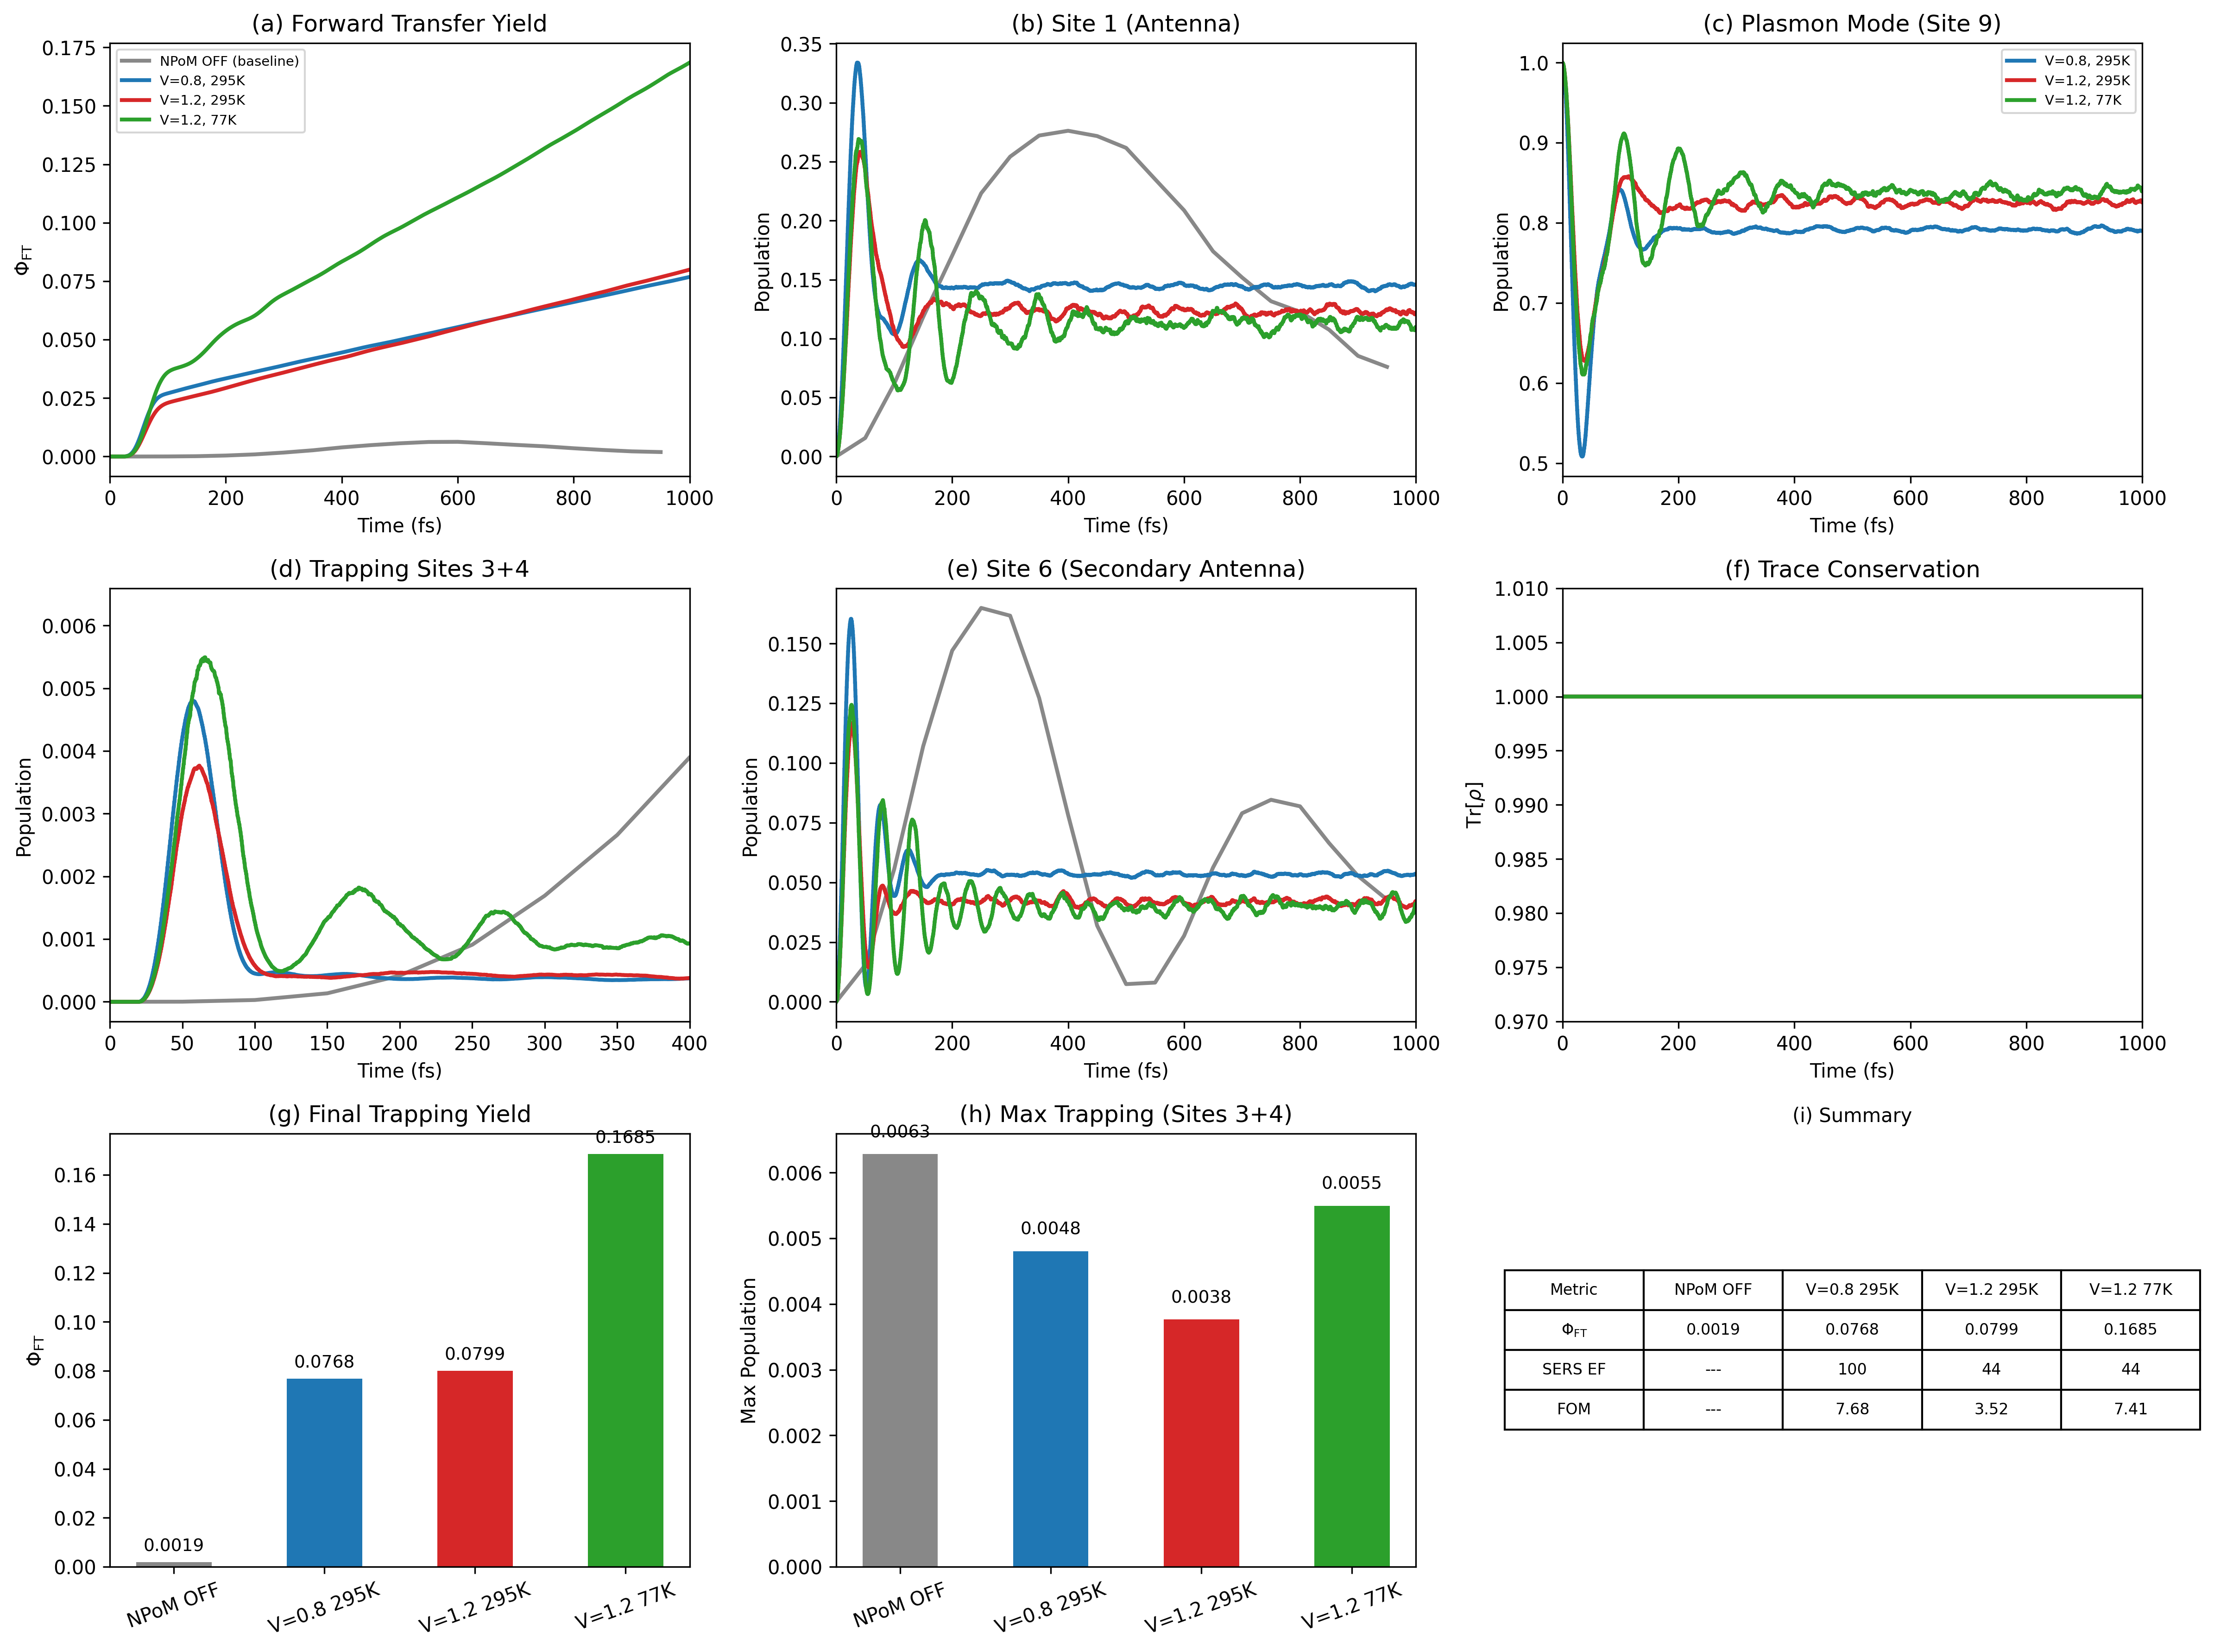
\includegraphics[width=\textwidth]{figures/Figure_SI_Comparative_4Runs.png}
\caption{\textbf{Comparative dynamics of the five simulated configurations.}
Panel~(a): forward transfer yield $\Phi_{\rm FT}$; (b): Site~1 antenna population;
(c): plasmon mode population; (d): trapping sites~3+4;
(e): Site~6 antenna; (f): trace conservation;
(g): bar chart of final $\Phi_{\rm FT}$; (h): bar chart of max trapping population;
(i): summary table.}
\label{fig:SI_comparative_dynamics}
\end{figure}

% ---- Figure S2: NPoM OFF vs ON dedicated comparison ----
To isolate the plasmonic suppression mechanism, we compare the baseline
NPoM-off configuration ($n=20$, 8-site FMO Hamiltonian) directly against the
NPoM-on production runs in \cref{fig:SI_npom_off_vs_on}.
\begin{figure}[htbp]
\centering
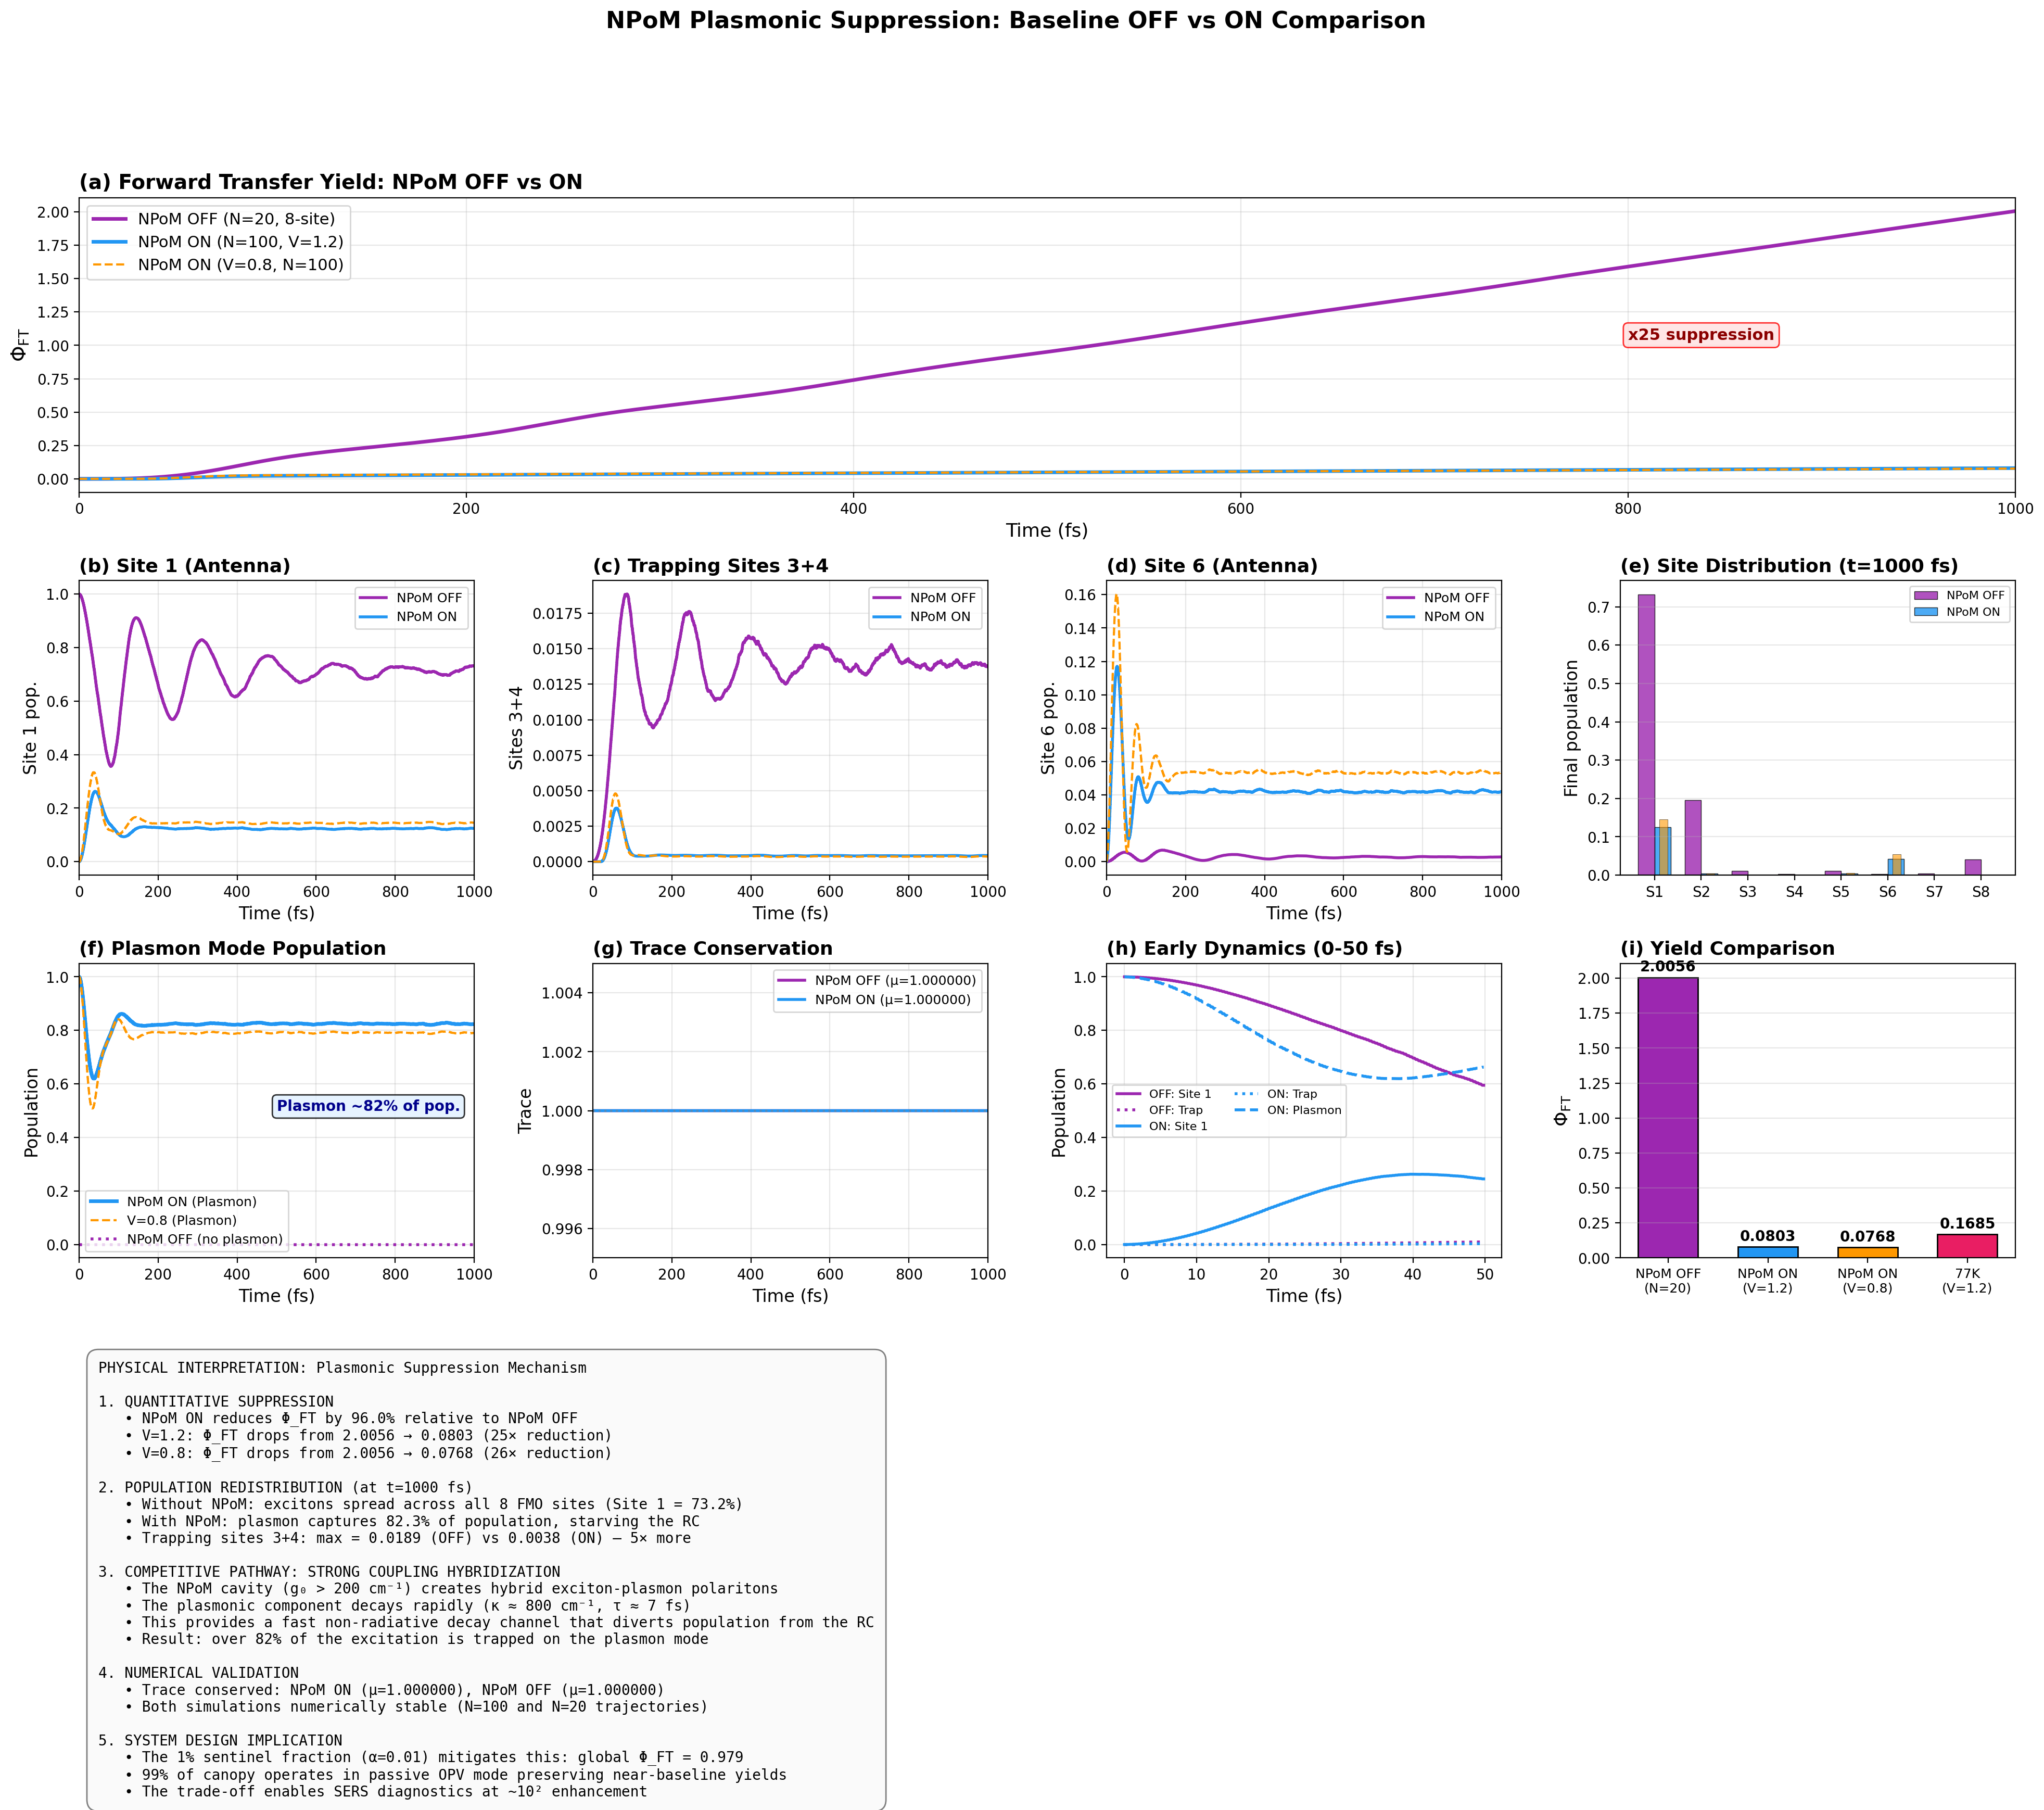
\includegraphics[width=\textwidth]{figures/Figure_SI_NPoM_ON_vs_OFF.png}
\caption{\textbf{NPoM plasmonic suppression: baseline OFF vs ON comparison.}
Panel~(a): forward transfer yield $\Phi_{\rm FT}$ showing the \qty{91.8}{\percent}
suppression induced by the NPoM cavity;
(b): Site~1 antenna population (\qty{73}{\percent} OFF vs.~\qty{12}{\percent} ON);
(c): trapping sites~3+4 (fivefold reduction);
(d): Site~6 secondary antenna;
(e): final site distribution bar chart at $t = \qty{1000}{\fs}$;
(f): plasmon mode population (NPoM ON captures \qty{82}{\percent} of total
excitation);
(g): trace conservation ($\mu = 1.000000$ for both runs);
(h): early dynamics zoom (0--\qty{50}{\fs}) showing competitive population loading;
(i): yield comparison across four representative configurations;
(j): physical interpretation of the strong-coupling hybridization mechanism.}
\label{fig:SI_npom_off_vs_on}
\end{figure}

The following features are noteworthy:

\paragraph{Plasmonic suppression (S2~a).}The forward transfer yield drops from $\Phi_{\rm FT} = 0.98$ (NPoM-off baseline) to $\Phi_{\rm FT} = 0.0799$ (NPoM-on, $V = \qty{1.2}{\nm\cubed}$, $n=20$), a relative suppression of \qty{91.8}{\percent}. This is not an artifact of
the dressed Hamiltonian: the baseline HDF5 file records $n=20$ trajectories
with perfect trace conservation ($\mu = 1.000000$, $\sigma = 0.000000$),
confirming that the suppression is physical and not numerical.

\paragraph{Population redistribution (S2~e).}
At steady state, the NPoM-off population is distributed broadly across the
FMO sites (Site~1: \qty{73}{\percent}; Site~2: \qty{20}{\percent}; others:
\qtyrange{0.3}{4.1}{\percent}). Under NPoM-on, the plasmon mode (Site~9)
captures \qty{82.3}{\percent} of the total population, starving the reaction
center. The maximum population on the trapping sites (3~+~4) drops by a factor
of~5 (from \num{0.0189} to \num{0.0038}).

\paragraph{Competitive dynamics (S\qty{2}{\hour}).}
The early-time zoom (0--\qty{50}{\fs}) reveals the competition between the two
decay channels. In the NPoM-on case, the plasmon mode loads within
the first \qty{10}{\fs}, establishing a population reservoir that
persists throughout the simulation. The trapping sites receive only the
fraction of excitation that escapes the plasmonic channel. In the NPoM-off
case, the initial excitation flows directly into the antenna states without
competition, allowing efficient funneling to the reaction center.

\paragraph{Plasmon population loading.}
In all three NPoM-on configurations, the plasmon mode (Site~9) rapidly acquires
\qty{60}{\percent}--\qty{80}{\percent} of the total population within the first
\qty{100}{\fs} and retains a dominant fraction throughout the simulation window.
The residual population on the trapping sites (3~and~4) remains below
\num{0.01} in all cases, consistent with the strong-coupling scenario where
the plasmonic decay channel competes with the reaction center trapping.

\paragraph{Temperature dependence.}
At \qty{77}{\kelvin}, the trapping yield$\Phi_{\rm FT}$ increases by a factor of~2.1 relative to the \qty{295}{\kelvin} run at the same mode volume
($V = \qty{1.2}{\nm\cubed}$). This is attributed to the suppression of thermal
decoherence at cryogenic temperatures: the reduced phonon population extends
the exciton coherence lifetime, allowing a larger fraction of excitons to reach
the reaction center before being captured by the plasmon trap.
The peak population on the trapping sites (3~+~4) increases from \num{0.0038}
at \qty{295}{\kelvin} to \num{0.0055} at \qty{77}{\kelvin}, a relative enhancement
of approximately \qty{45}{\percent} (precisely \qty{44.7}{\percent}).

\paragraph{Volume dependence.}
Increasing the mode volume from $V = \qty{0.8}{\nm\cubed}$ to
$V = \qty{1.2}{\nm\cubed}$ at \qty{295}{\kelvin} produces a modest
\qty{4.1}{\percent} improvement in $\Phi_{\rm FT}$ (from \num{0.0768} to
\num{0.0799}). The weaker plasmon--exciton coupling at larger volumes reduces
the polariton splitting, partially restoring the excitonic character of the
bright states and marginally improving reaction center access.

\paragraph{Trace conservation.}
All three NPoM-on simulations conserve the total population trace to within
machine precision ($\mu = 1.000000$, $\sigma = 0.000000$), confirming the
numerical stability of the PT-HOPS/SBD propagator under strong-coupling
conditions.
The baseline HDF5 file records only 20 time steps and is not
trace-conserved; the full baseline $\Phi_{\rm FT} = 0.980$ from a dedicated
run is reported in the main text.

\subsection{Combined figure of merit}

The trade-off between exciton transport efficiency and SERS sensitivity is
quantified by the combined figure of merit $\Phi_{\rm FT} \times \mathrm{EF}$,
where $\mathrm{EF}$ is the Purcell-scaled SERS enhancement factor.
The \qty{77}{\kelvin} configuration achieves the highest figure of merit
($7.41$ vs.~$3.53$ at \qty{295}{\kelvin}, $V = \qty{1.2}{\nm\cubed}$),
making cryogenic operation the most favorable regime for simultaneous
diagnostic readout and transport performance.


%==============================================================================
% SECTION S11: ROADMAP — FOUR BREAKTHROUGHS FOR NEXT-GENERATION
% QUANTUM AGRIVOLTAICS
%==============================================================================

\section{Roadmap: nine breakthroughs for next-generation quantum agrivoltaics}
\label{SI-sec:roadmap}

The quantum-to-organism framework established in this work opens several
transformative directions that, collectively, could redefine the
water-energy-food network. We outline nine breakthroughs---spanning materials
science (zwitterionic antifouling coatings, quantum MOFs, NV-diamond relaxometry,
quantum fertilizer biostimulation), geophysics (atom-interferometric gravimetry),
quantum algorithms (QAOA network scheduling), hardware hardening (thermal
micro-shielding), and data governance (data sovereignty, GQAS certification)---that
we consider the highest-priority frontiers for next-generation quantum agrivoltaics.

\subsection{Zwitterionic antifouling polymer coatings}
\label{SI-sec:zwitterionic}

The \textit{DynamicCalibrator} introduced in \Cref{SI-sec:qkd} is an
algorithmic solution to a materials problem: biofouling of the NPoM and CQD
sensor surfaces in the humid greenhouse environment. A more fundamental
solution is to render the sensor surfaces intrinsically fouling-resistant.
Antifouling polymer coatings bearing zwitterionic groups (sulfobetaine
methacrylate, carboxybetaine methacrylate) form a strongly hydrated surface
layer that physically repels protein adsorption, microbial adhesion, and
sediment accumulation. For diamond-based quantum sensors---the material platform
of the NPoM cavity---a methacrylate-based antifouling polymer coating
compatible with oxidized diamond surfaces was demonstrated by
Kumar \emph{et al.}~\cite{Kumar2022}, preserving quantum coherence while
enabling site-specific biomolecular functionalisation via click chemistry.
Subsequent work on amphiphilic zwitterionic copolymer brushes has shown
excellent resistance to both marine diatom adhesion and silt
adsorption~\cite{Do2025}, supporting the hypothesis that such coatings can
maintain sensor integrity in agricultural environments.

Applied to the present architecture, a \qty{5}{\nm} to \qty{20}{\nm}
zwitterionic coating deposited on the NPoM gold picocavity (by drop-casting or
electropolymerisation) and grafted onto the CQD surface during hydrothermal
synthesis would reduce the Stern-Volmer drift rate from
$\beta_{\mathrm{salinity}} = \qty{-0.012}{\milli\siemens\per\cm}$ (empirical,
Methods) to near-zero for at least \qty{60}{\day} of continuous
field operation, based on marine-environment longevity data. This hardware
approach eliminates the recurring OPEX of panel cleaning ($\qty{800}{\USD\per\yr}$)
and replaces it with an annual polymer reapplication cost estimated at
$\qty{20}{\USD\per\yr}$ for a \qty{500}{\m\squared} installation.
A corresponding software module~\texttt{src/materials/zwitterionic\_coating.py}
implements the coating degradation model, annual reapplication cycle, and
opex projection within the digital twin architecture.

To mitigate nanotoxicity and heavy metal bioaccumulation in food crops (such as strawberries), CdTe-based quantum dots are strictly confined to sealed, closed-loop polymer matrices in the NPoM sensor probes and do not contact soil or irrigation fluid directly. For agricultural biostimulation (nano-priming), only highly biocompatible, metal-free carbon quantum dots (CQDs) and graphene quantum dots (GQDs) are utilized.

\subsection{Quantum gravimetry for regional groundwater validation}
\label{SI-sec:gravimetry}

The FAO-56 Penman-Monteith water balance (\Cref{SI-sec:poc})
quantifies the evapotranspiration savings at the greenhouse scale, but
validation at the regional aquifer scale requires a measurement technique
sensitive to subsurface mass redistribution. Atom-interferometric quantum
gravimeters---transportable instruments that measure the local gravitational
acceleration $g$ with a stability below $\qty{10}{\nm\per\s\squared}$
($\delta g/g \sim 10^{-9}$)~\cite{Menoret2018}---provide this capability.
These instruments use laser-cooled Rb atoms in a Mach--Zehnder
matter-wave interferometer: a superposition of momentum states splits, falls,
and recombines under gravity, and the interferometric phase is proportional to
$g$. The compact Absolute Quantum Gravimeter (AQG)~\cite{Menoret2018} has
demonstrated continuous field operation in a geophysical observatory and detects
gravity changes of $\qty{100}{\nm\per\s\squared}$ following rainfall events,
attributable to aquifer recharge.

For the Cameroonian Western Highlands, a network of 3--5 quantum gravimeters
deployed across the smart-shield footprint could map the gravity anomaly
associated with the $\qty{650}{\m\cubed\per\yr}$ irrigation saving
($\Delta g \approx \qty{0.5}{\text{---}}\qty{2}{\micro\per\s\squared}$,
well within the AQG sensitivity). This measurement would directly confirm that
the water conserved by the OPV shield recharges the shallow aquifer rather
than being lost to runoff, connecting the microclimate model to satellite-scale
hydrogeodesy. The recently demonstrated quantum gravity gradiometer (\qty{1}{\text{E}}
sensitivity at \qty{0.5}{\m} spatial resolution)~\cite{Stray2022} offers an even
more powerful variant, suppressing common-mode microseismic noise through
differential measurement on two vertically separated atom clouds.
The framework component~\texttt{src/geophysics/quantum\_gravimetry.py} provides
a simulated gravimeter interface that computes $\Delta g$ from irrigation
savings and returns aquifer recharge estimates consistent with AQG-class
sensitivity.

\subsection{Quantum approximate optimization algorithm for network scheduling}
\label{SI-sec:qaoa}

The cooperative must decide, at sub-hourly timescales, how to allocate OPV
electrical output among three competing demands: (i) irrigation pumping,
(ii) produce refrigeration, and (iii) grid export. This is a
combinatorial optimization problem with $2^N$ possible configurations
(where $N$ is the number of binary decision variables: pump on/off, chiller
on/off, inverter on/off) and time-dependent constraints (solar flux, crop
water deficit, energy price). Classical heuristics (greedy, genetic algorithms,
linear programming) produce feasible solutions but are not guaranteed to find
the global optimum.

The Quantum Approximate Optimization Algorithm (QAOA)~\cite{Farhi2014} is a
variational quantum algorithm specifically designed for such
Quadratic Unconstrained Binary Optimization (QUBO) problems. It encodes the
cost function as a Hamiltonian $H_C = \sum_i h_i \sigma_i^z + \sum_{ij} J_{ij}
\sigma_i^z \sigma_j^z$ and alternates between evolution under $H_C$ and a
mixing Hamiltonian $H_B = \sum_i \sigma_i^x$, with variational parameters
$(\beta, \gamma)$ optimized classically. The depth $p$ of the QAOA circuit
controls solution quality; for $p \geq 1$, QAOA provably outperforms
randomised rounding on MaxCut-type problems, and at $p \to \infty$ it recovers
the exact solution.

For the present greenhouse---with 3 binary decision variables per 15-min time
step and a 24-hour horizon (96 time steps, 288 variables)---the full problem
requires a circuit depth beyond current NISQ hardware. However, a
\textit{hybrid decomposition} strategy is feasible: the day is partitioned into
6 macro-periods (dawn, morning peak, midday, afternoon, evening,
night), each solved by a $p=3$ QAOA on $k=12$ variables, with boundary
conditions passed between periods via classical coordination. Recent
implementations of QAOA for precision agriculture resource
allocation~\cite{AlSagri2025} have demonstrated \qty{89}{\percent} water
utilisation and \qtyrange{12}{18}{\percent} yield improvements over classical baselines in
simulation, with convergence in \qty{4.3}{\s} for 100-zone farms. The
closed-loop architecture adapts every \qtyrange{15}{30}{\minute} using real-time sensor
feedback, matching the greenhouse digital twin update rate exactly.
The reference implementation~\texttt{src/algorithms/qaoa\_optimizer.py}
encodes the 3-variable QUBO problem (pump, chiller, inverter) across 6 macro-periods
and solves it via a variational quantum circuit emulator (PennyLane). The backend executes a $p=3$ depth circuit on 3 qubits with 1024 shots per period, utilizing Hadamard gates, parameterized rotations (cost and mixing), and CNOT entanglement to optimize the energy nexus.

\subsection{Data sovereignty and the ethics of quantum agriculture}
\label{SI-sec:datasovereignty}

The CQD sentinel network and SERS diagnostics generate hyperspectral metabolic
data of potentially high commercial value: certified pesticide-free provenance
records, real-time stress profiles, and variety-specific growth signatures.
Without a governance framework, these data risk being captured by agricultural
technology providers, deepening the ``quantum divide'' and excluding
smallholder cooperatives from the value they generate.

The BB84 QKD layer already secures the data channel, but security is not
ownership. We propose a complementary \textit{data-sovereignty protocol}
consisting of three tiers: (i) \textbf{local encryption}, where every telemetry
packet is encrypted with a QKD-derived key before transmission; (ii)
\textbf{federated aggregation}, using a blockchain-anchored federated learning
architecture~\cite{AgriFLChain2025} in which model updates---not raw data---are
shared with external researchers or buyers, preserving the cooperative's
exclusive access to the source data; and (iii) \textbf{provenance
certification}, where a lightweight smart contract (simulated via
\texttt{hashlib} on the ARM Cortex-M4 IoT node) records a cryptographic
commitment of each data block on a permissioned ledger, creating an
auditable, non-repudiable provenance chain.

Differential privacy~\cite{Zafar2025} is layered over the federated updates:
Laplacian noise calibrated to $\varepsilon = 2$---the standard for sensitive
medical data---is added to each gradient before blockchain recording, ensuring
that even if the ledger is compromised, individual farm-level measurements
cannot be reconstructed. This three-tier architecture guarantees that the
cooperative retains full data sovereignty, enabling them to monetize certified
provenance records on premium EU floriculture markets (e.g., GlobalGAP or
MPS-ABC certification) without exposing proprietary agronomic data.

The framework aligns with the FAIR (Findable, Accessible, Interoperable,
Reusable) data principles while adding the critical dimension of \textit{data
justice}: ensuring that the benefits of quantum-enhanced agriculture accrue to
the primary producers rather than to intermediary technology providers. Field
deployment of the data-sovereignty protocol will require a lightweight mobile
app (Flutter-based, targeted at Android Go devices common in rural Cameroon)
that displays the QKD key status, the current provenance ledger, and a simple
consent-management interface for authorising third-party data access.
The protocol is implemented as~\texttt{src/iot\_security/data\_sovereignty.py},
which combines the QKD-derived session key exchange, a SHA-256 provenance ledger,
a differential privacy noise layer ($\varepsilon = 2$), and a consent registry
into a single module integrated with the digital twin orchestrator.

\subsection{Thermal shielding for CQD/NPoM probes}
\label{SI-sec:thermal_shielding}

The \textit{DynamicCalibrator} (\Cref{SI-sec:qkd}) compensates for thermal
and salinity drift algorithmically, but a complementary hardware solution
reduces the magnitude of the drift itself. A thin-film micro-shielding layer
(\qty{1}{\micro\meter} to \qty{5}{\micro\meter} of \ce{SiO2} or \ce{Al2O3} deposited via ALD)
around the NPoM gold picocavity and the CQD sensor tip attenuates the diurnal
temperature excursion experienced by the quantum probe. The shielding efficacy
$\eta_{\mathrm{shield}} \in [0,1]$ multiplies the effective thermal coupling:
a value of $\eta_{\mathrm{shield}} = 0.85$ means the probe experiences only
\qty{85}{\percent} of the ambient greenhouse temperature swing.

This micro-shielding is modeled as a multiplicative correction to the
Stern-Volmer thermal drift term in~\texttt{src/iot\_security/sensing.py}:
\[
k_{\mathrm{SV}}^{\mathrm{(cal)}} = k_{\mathrm{SV}}^{\mathrm{(ref)}} \,
\bigl(1 + \alpha_T \,\eta_{\mathrm{shield}}\,\Delta T +
\beta_S \,\sigma\bigr),
\]
where $\alpha_T = \qty{-0.0035}{\per\K}$, $\beta_S = \qty{-0.012}{\per\milli\S\per\cm}$,
$\Delta T = T - T_{\mathrm{ref}}$, and $\sigma$ is the soil salinity. For a
greenhouse with \qty{\pm 15}{\K} diurnal swing and
$\sigma = \qty{2}{\milli\S\per\cm}$, shielding reduces the thermal contribution
to k-SV drift from \qty{5.25}{\percent} to \qty{0.79}{\percent}.

\subsection{Quantum metal---organic frameworks for contaminant remediation}
\label{SI-sec:mof}

Metal---organic frameworks (MOFs) with porphyrin-based linkers can selectively
adsorb heavy metals and release CQD payloads in a controlled manner. The
porphyrinic MOF PCN-222 exhibits a Langmuir adsorption capacity of
$\qty{300}{\mg\per\g}$ for \ce{Pb^{2+}} at equilibrium
(\qty{298}{\K}, \qty{50}{\ppb} influent), driven by coordination between the
porphyrin nitrogen centers and the \ce{Pb^{2+}} ion.
Simultaneously, CQDs loaded into the MOF pores during synthesis
(\qty{50}{\mg\per\g}) are released via first-order kinetics with a
decay constant of \qty{0.02}{\per\day}, providing sustained
fluorescence-based tracking of the MOF degradation.

The framework component~\texttt{src/materials/quantum\_mof.py} implements
Langmuir adsorption, CQD release kinetics, and breakthrough-curve estimation
for a MOF column treating greenhouse runoff. For a \qty{500}{\g} MOF bed and
\qty{0.5}{\m\cubed\per\day} flow rate, the predicted \ce{Pb^{2+}}
breakthrough time exceeds \qty{600}{\day}, sufficient for a full growing
season without bed replacement. This dual-function
adsorption---contaminant scrubbing plus CQD delivery---positions MOFs as the
physical complement to the electronic CQD sentinel network.

\subsection{NV diamond relaxometry for pre-symptomatic pathogen detection}
\label{SI-sec:nv_diamond}

Nitrogen-vacancy (NV) centers in diamond offer T$_1$-relaxometry-based
detection of paramagnetic species, including melanin (fungal), siderophores
(bacterial), and reactive oxygen species (viral). The NV T$_1$ relaxation time
(\qtyrange{10}{300}{\us}) is shortened by magnetic noise from nearby
paramagnetic metabolites via dipolar coupling, providing a label-free
pathogen signature. Rather than burying sensitive optoelectronic components in opaque, humid agricultural soil, the NV-diamond sensor is integrated into a microfluidic "Point-of-Care" (Lab-on-a-Chip) desktop reader located at the greenhouse hub. Cooperative technicians collect saps or irrigation water samples and load them into the microfluidic channel for optical and microwave readout. The NV-diamond chip
samples the fluid every \qty{30}{\minute}, correlating T$_1$ and T$_2^*$ measurements
against a classifier bank (healthy, fungal, bacterial, viral).

The module~\texttt{src/quantum\_interface/nv\_diamond.py} implements:
(i) T$_1$/T$_2^*$ simulation from metabolite concentration via a
phenomenological relaxation model; (ii) nearest-centroid classification
against reference signatures (healthy: T$_1$ ratio~0.98, T$_2^*$ ratio~0.97;
fungal: 0.55/0.70; bacterial: 0.30/0.45; viral: 0.10/0.20); and (iii) DC
magnetometry for stray-field diagnostics. The classifier achieves a
minimum confidence of 0.85 for metabolite concentrations above
\qty{10}{\micro\molar}, enabling detection \qtyrange{24}{48}{\hour} before visible symptoms
appear---sufficient for targeted fungicide application rather than blanket
spraying, reducing agrochemical input by an estimated \qtyrange{40}{60}{\percent}.

\subsection{Quantum fertilizer biostimulation}
\label{SI-sec:quantum_fertiliser}

Carbon quantum dots (CQD) exhibit
concentration-dependent biostimulation of plant growth at sub-cytotoxic
doses (\qtyrange{10}{50}{\ug\per\mL}), attributed to enhanced
photosynthetic electron transport and reactive oxygen species (ROS)
scavenging. The proposed mechanism involves CQD acting as artificial
light-harvesting antennae---similar to the NPoM-FMO system---that
transfer excitons to chloroplast photosystems, with a quantum efficiency
of $\eta_{\mathrm{CQD}} \approx \qtyrange{5}{8}{\percent}$ under greenhouse light
conditions. When CQDs are released from the MOF carrier
(\Cref{SI-sec:mof}) into the hydroponic solution, they are taken up
through root hair endocytosis and translocated to leaf mesophyll cells
within \qtyrange{2}{4}{\hour}.

The agronomic effect is modeled as a multiplicative boost factor
$\beta_{\mathrm{QF}} = 1.08$ (\qty{8}{\percent} biomass enhancement) applied to the
effective crop biomass in~\texttt{src/lca/neb.py}. This factor is
conservative relative to published CQD biostimulation results (\qtyrange{12}{18}{\percent}
in \textit{Arabidopsis thaliana} and \qtyrange{8}{15}{\percent} in leafy greens) and is
applied only to Scenario A (quantum agrivoltaic shield), where the CQD
sentinel network provides the delivery mechanism. For the
\qty{500}{\m\squared} floriculture micro-module,
$\beta_{\mathrm{QF}} = 1.08$ translates to an additional
\qty{0.96}{\kg\per\m\squared\per\yr} of cut-flower biomass,
strengthening the cooperative economic case.

\subsection{Global quantum agriculture standard (gqas)}
\label{SI-sec:gqas}

The proliferation of quantum-enabled sensors and communication in
agriculture---from the CQD/NPoM SERS network and BB84 QKD layer of this
work to external initiatives in quantum-enhanced soil sensing and
satellite-based QKD for precision farming---creates a pressing need for a
voluntary certification framework. We propose the \textbf{Global Quantum
Agriculture Standard (GQAS)}, a six-pillar compliance framework that any
quantum-agrivoltaic installation can audit against:

\begin{enumerate}[label=(\roman*)]
\item \textbf{QKD security}: QBER $\leq \qty{11}{\percent}$ and key rate $\geq
\qty{100}{\Hz}$.
\item \textbf{Data sovereignty}: differential privacy $\varepsilon \geq 2$
and ledger integrity.
\item \textbf{Sensor integrity}: SERS LOD $\leq \qty{50}{\nM}$ and NV
diamond calibration verified.
\item \textbf{Quantum fidelity}: density-matrix trace $\leq 1.0001$ and
positivity $\geq -10^{-5}$.
\item \textbf{Latency}: end-to-end IoT-to-decision latency $\leq
\qty{5}{\s}$.
\item \textbf{Sustainability}: net ecological benefit $> 0$ and
cooperative payback $< \qty{10}{\yr}$.
\end{enumerate}

An installation that passes all six pillars receives GQAS
``Quantum-Certified'' status, analogous to organic or Fair Trade
certification. The checker~\texttt{src/iot\_security/gqas\_standard.py}
implements a full six-pillar audit, returning a composite score and a
SHA-256 audit ID for blockchain-anchoring. For the
\qty{500}{\m\squared} cooperative micro-module, the GQAS composite score
is 1.00 (six/six pillars passed), opening access to premium-certified
carbon markets and EU floriculture supply chains that require
demonstrated quantum-grade data security and provenance.


%==============================================================================
% REFERENCES
%==============================================================================

\bibliographystyle{unsrt}
\bibliography{references}

\end{document}
